\subsection{Emulation}

In addition to the gate-level simulation, an emulator is written. This emulator provides a software interface to an implementation of the \ac{isa}. Through this interface, the full internal state can be read out at any stage of program execution. This allows comprehensive testing, which is not possible in the simulation software since it has no way to hook into the internal state using a programming language. The emulation is written as close as possible to its gate-level counterpart. By doing so, testing within the emulator also verifies the behavior of the simulator to some extent. \\

The emulator is implemented in the Rust programming language. This language was chosen due to previous experience of the author. Other suitable candidates are C or C++, as well as other relatively low-level languages such as Zig. Writing an emulator requires modelling of hardware. Therefore, the hardware must be accurately described on a bit-by-bit or gate-by-gate basis. For this reason, languages such as Java offer too high of a level of abstraction from the primitive types of sized integers. \\

The software simulator processes instructions using a simulated clock input. This level of granularity of simulation is deemed sufficient for testing and verification of the behavior of the implementation. It is possible to enable more granular testing by subdividing a single clock cycle into the theoretical signal propagation phases. Going even further, it is possible to simulate the physical properties of the materials used in an implementation, which enables testing of propagation times, edge transition times etc. However, this kind of analog analysis is outside of the scope of this work, as the device will only be operated at low clock speeds. Therefore, the emulator at its core works by repeatedly applying a transition function to the internal state, which results in a new internal state. The internal state is given by the state of all memories of the device at any one point in time. All other elements are stateless as they consist of combinatorial circuits.

\begin{align}
    S_{RAM}            &= \left\{ X_n \;\middle|\; X_n \in \mathcal{B}^8,    \; 0 \leq n < 2^{16} \right\} \nonumber \\
    S_{OpROM}          &= \left\{ X_n \;\middle|\; X_n \in \mathcal{B}^{32}, \; 0 \leq n < 2^{16} \right\} \nonumber \\
    S_{ControlROM}     &= \left\{ X_n \;\middle|\; X_n \in \mathcal{B}^{16}, \; 0 \leq n < 2^{7}  \right\} \nonumber \\
    S_{Registers}      &= \left\{ X_n \;\middle|\; X_n \in \mathcal{B}^8,    \; 0 \leq n < 7      \right\} \nonumber \\
    S_{ProgramCounter} &= X \in \mathcal{B}^{16} \nonumber  \\
    S_{Halted}         &= X \in \mathcal{B}      \nonumber  \\
    S &= (S_{RAM}, S_{OpROM}, \ldots , S_{Halted}) \nonumber
\end{align}
\captionof{figure}{Constituents of the internal state of the emulator}
\label{align:emulation_internal_state}


\begin{figure}[h!]
    \centering
    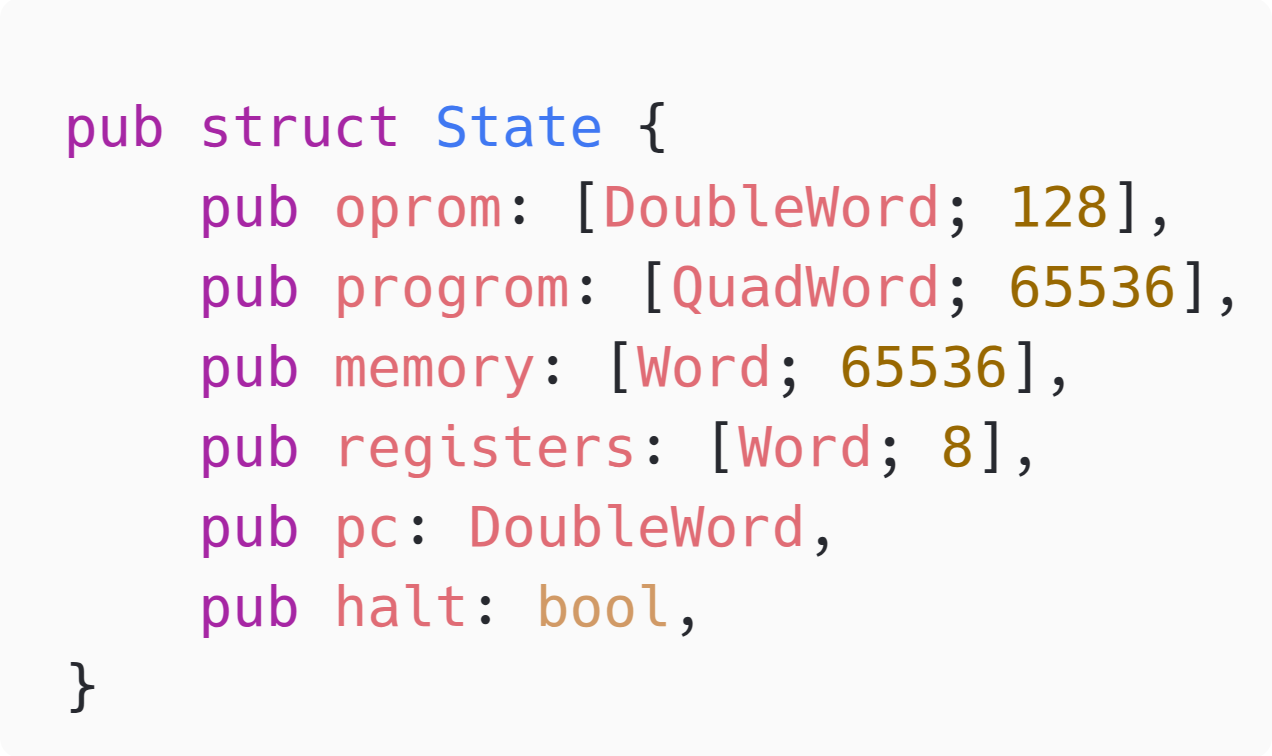
\includegraphics[width=0.48\textwidth]{images/rust_emulator_state_datatype.png}
    \caption{Rust representation of the emulator state as a struct datatype}
    \label{fig:rust_datatype_emulator_state}
\end{figure}

\autoref{align:emulation_internal_state} shows the individual components of the internal state, as well as the tuple consisting of all of them denoted as $S$\footnote{The device state has a total of 2622537 bits, which results in a total of $2^{2622537}$ different states}. This type is translated directly into its Rust counterpart. While Rust supports tuples, the type is instead captured as a struct, which additionally allows naming the individual fields for easier access. \autoref{fig:rust_datatype_emulator_state} shows this datatype. A constructor is implemented, which initializes all fields to 0. Another function allows loading binary program files as well as a binary file that represents the control signal memory. This is equivalent to resetting the state of the \ac{cpu}, clearing all registers, while the contents of all \acp{rom} remain intact. \\

A core ``tick'' function to transition from one state to another is implemented with the signature $ T \colon S \xrightarrow{} S $. Within this function, the execution of a single instruction cycle is implemented. The function first fetches the current instruction by indexing into the instruction memory using the current program counter. Then, this instruction is propagated through all combinatorial circuits. When the state of all signals after propagating the current state is known, the next state can be constructed and returned as a result. \\

Like the simulation, the emulation tests and verifies a design on the level of individual logic gates. For this reason, all combinatorial circuits are implemented exactly as they are built in the simulation. The Rust program consists of multiple boolean functions, all of which have the signature 

$$ \mathcal{B}^n \xrightarrow{}  \mathcal{B}^m \mid n, m \in \mathbb{N}^* $$

To distinguish multiple inputs and outputs and assign meaningful names to them in the source code, the input and output data may be split up into multiple smaller data, giving the signature 

\begin{gather*}
    I_0 \times I_1 \times \ldots \times I_n \xrightarrow{} (O_0, O_1, \ldots, O_m) \\
    \\
    I_x \in \mathcal{B}^{n_x}, O_y \in \mathcal{B}^{m_y} \\
    0 \leq x \leq n, 0 \leq y \leq m \\
    n_x, m_y, n, m \in \mathbb{N}^*
\end{gather*}

\begin{figure}[h!]
    \centering
    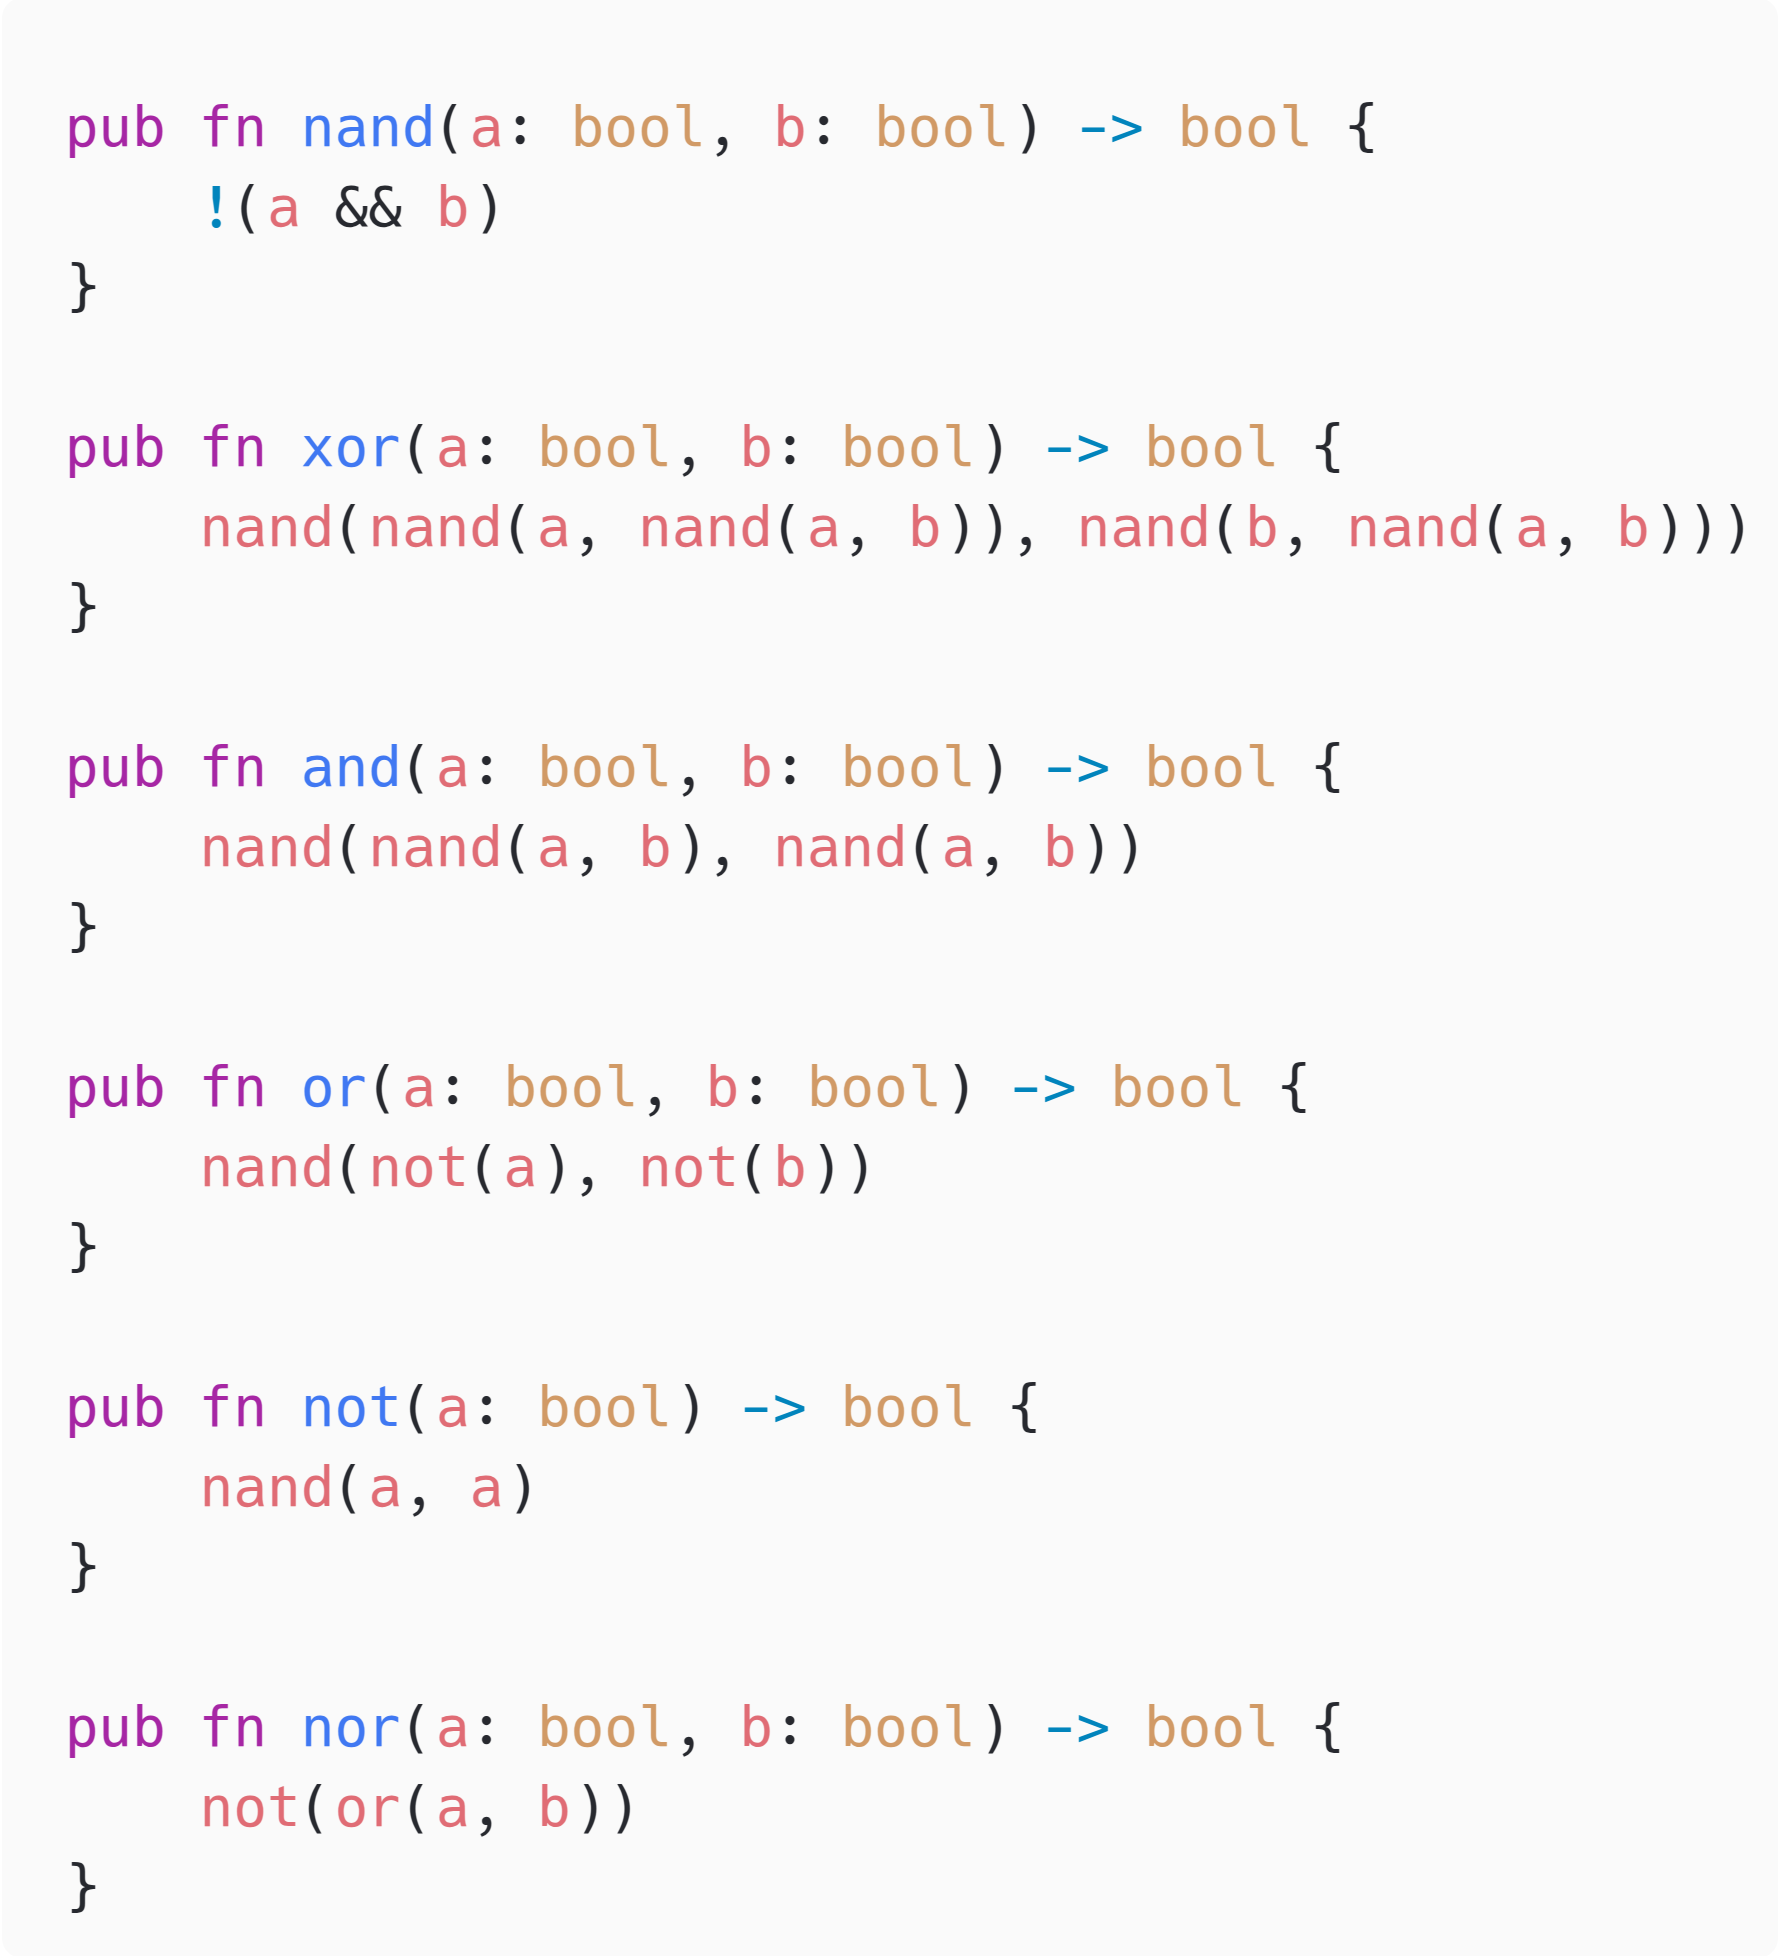
\includegraphics[width=0.48\textwidth]{images/rust_basic_logic_operators.png}
    \caption{Rust implementation of the logic gate operators \texttt{NAND, XOR, AND, OR, NOT, NOR} using only the operations \texttt{!} and \texttt{\&\&}}
    \label{fig:rust_basic_boolean_operators}
\end{figure}

\autoref{fig:rust_basic_boolean_operators} shows the implementation of the fundamental \texttt{NAND} gate using only the operations \texttt{!} and \texttt{\&\&}, as well as other fundamental boolean operators from only the \texttt{NAND} gate. All functions shown have the signature $ \mathcal{B} \times \mathcal{B} \xrightarrow{} \mathcal{B} $, except for the unary \texttt{NOT} operator, which has only one input. From these basic functions, all other combinatorial circuits are built.  \\

The highest level functions represent the logical modules described in \autoref{sec:implementation_logical}, where the signature of each function directly matches the number of inputs and outputs of the module. During and after the implementation, several test cases are implemented, where in each test case, a predefined input is compared to the expected output of such a combinatorial boolean function. The results are cross-checked with the results of the individual modules in the simulator. The combinatorial functions serve as the building blocks for signal propagation within the ``tick'' function. The fields of the state data structure serve as the non-combinatorial, i.e synchronous sections of the gate design.

